\documentclass[12pt,english]{article}\usepackage[]{graphicx}\usepackage[usenames, dvipsnames]{xcolor}
% maxwidth is the original width if it is less than linewidth
% otherwise use linewidth (to make sure the graphics do not exceed the margin)
\makeatletter
\def\maxwidth{ %
  \ifdim\Gin@nat@width>\linewidth
    \linewidth
  \else
    \Gin@nat@width
  \fi
}
\makeatother

\definecolor{fgcolor}{rgb}{0.345, 0.345, 0.345}
\newcommand{\hlnum}[1]{\textcolor[rgb]{0.686,0.059,0.569}{#1}}%
\newcommand{\hlstr}[1]{\textcolor[rgb]{0.192,0.494,0.8}{#1}}%
\newcommand{\hlcom}[1]{\textcolor[rgb]{0.678,0.584,0.686}{\textit{#1}}}%
\newcommand{\hlopt}[1]{\textcolor[rgb]{0,0,0}{#1}}%
\newcommand{\hlstd}[1]{\textcolor[rgb]{0.345,0.345,0.345}{#1}}%
\newcommand{\hlkwa}[1]{\textcolor[rgb]{0.161,0.373,0.58}{\textbf{#1}}}%
\newcommand{\hlkwb}[1]{\textcolor[rgb]{0.69,0.353,0.396}{#1}}%
\newcommand{\hlkwc}[1]{\textcolor[rgb]{0.333,0.667,0.333}{#1}}%
\newcommand{\hlkwd}[1]{\textcolor[rgb]{0.737,0.353,0.396}{\textbf{#1}}}%
\let\hlipl\hlkwb

\usepackage{framed}
\makeatletter
\newenvironment{kframe}{%
 \def\at@end@of@kframe{}%
 \ifinner\ifhmode%
  \def\at@end@of@kframe{\end{minipage}}%
  \begin{minipage}{\columnwidth}%
 \fi\fi%
 \def\FrameCommand##1{\hskip\@totalleftmargin \hskip-\fboxsep
 \colorbox{shadecolor}{##1}\hskip-\fboxsep
     % There is no \\@totalrightmargin, so:
     \hskip-\linewidth \hskip-\@totalleftmargin \hskip\columnwidth}%
 \MakeFramed {\advance\hsize-\width
   \@totalleftmargin\z@ \linewidth\hsize
   \@setminipage}}%
 {\par\unskip\endMakeFramed%
 \at@end@of@kframe}
\makeatother

\definecolor{shadecolor}{rgb}{.97, .97, .97}
\definecolor{messagecolor}{rgb}{0, 0, 0}
\definecolor{warningcolor}{rgb}{1, 0, 1}
\definecolor{errorcolor}{rgb}{1, 0, 0}
\newenvironment{knitrout}{}{} % an empty environment to be redefined in TeX

\usepackage{alltt}
\usepackage[usenames, dvipsnames]{xcolor}
\usepackage[top=2cm, bottom=2cm, left=2.5cm, right=2.5cm]{geometry}
\usepackage[T1]{fontenc}
\usepackage{inputenc}
\usepackage{caption}
\usepackage{booktabs}
\setlength{\heavyrulewidth}{0.2em}
\usepackage{graphicx}
\usepackage{parskip}
\setlength{\parindent}{0pt}
\usepackage{amsmath}
\usepackage{url}
\usepackage[bookmarksnumbered]{hyperref}
\hypersetup{colorlinks, citecolor=RoyalBlue, linkcolor=RubineRed, urlcolor=MidnightBlue}
\hypersetup{pdfauthor={Constantin Manuel Bosancianu},
pdftitle={Two-level MLM},
pdfsubject={Two-level MLM specifications},
pdfkeywords={SSMT, 2019, MLM, tutorial, interpretation}}
\usepackage{babel}
\usepackage{CormorantGaramond}
\usepackage{dcolumn}
\usepackage{setspace}
\onehalfspacing
\usepackage{titlesec}
\titleformat{\section}{\large\bfseries}{\thesection}{0.4em}{}
\titleformat{\subsection}{\normalfont\bfseries}{\thesubsection}{0.2em}{}
\usepackage{apacite}
\bibliographystyle{apacite}
\makeatletter
\renewcommand{\maketitle}{
  \begin{flushleft}
    {\huge\@title}\\
    \vspace{10pt}
    {\large\@author}\\
    {\@date}
    \vspace{40pt}
  \end{flushleft}
}
\makeatother
\usepackage{afterpage}
% End of huxtable requirements
\usepackage{authblk}
\title{\textsc{Two-level MLM}}
\author{Constantin Manuel Bosancianu\footnote{You can reach me at \href{mailto:bosancianu@icloud.com}{bosancianu@icloud.com}. If you spot any mistakes I'd be grateful if you sent me an email pointing it out; I'll update the document and credit the help offered.}}
\affil{WZB Berlin Social Science Center \\ \textit{Institutions and Political Inequality}}
\date{\today}
\IfFileExists{upquote.sty}{\usepackage{upquote}}{}
\begin{document}
\maketitle

The current tutorial goes through the steps of running in R a standard two-level mixed-effects model. The data set used throughout is the one you are also working on for your assignment: the 6th wave of the European Social Survey, with a sample of 23 countries and a bit over 44,000 respondents.

First, read the data in \texttt{R} (please replace the working directory with the folder path on your machine). You can get a rough idea of what the variables in the data set measure, and how they are coded, by looking at the codebook for the ESS data, which has also been uploaded here.




\begin{knitrout}
\definecolor{shadecolor}{rgb}{0.969, 0.969, 0.969}\color{fgcolor}\begin{kframe}
\begin{alltt}
\hlstd{df_ess} \hlkwb{<-} \hlkwd{read.table}\hlstd{(}\hlkwc{file} \hlstd{=} \hlstr{"../../02-Data/ess.tsv"}\hlstd{,}
                     \hlkwc{header} \hlstd{=} \hlnum{TRUE}\hlstd{)}
\hlstd{df_ess}\hlopt{$}\hlstd{trustind} \hlkwb{<-} \hlkwd{rowMeans}\hlstd{(df_ess[,} \hlkwd{c}\hlstd{(}\hlstr{"ppltrst"}\hlstd{,} \hlstr{"pplfair"}\hlstd{,} \hlstr{"pplhlp"}\hlstd{)],}
                            \hlkwc{na.rm} \hlstd{=} \hlnum{TRUE}\hlstd{)}
\end{alltt}
\end{kframe}
\end{knitrout}

As dependent variable, I will be using a simple index of pro-social attitudes, which I've constructed here as a simple average of the three variables present in the data set: \textbf{\texttt{ppltrst}} (``most people can be trusted''), \textbf{\texttt{pplfair}} (``most people try to be fair''), and \textbf{\texttt{pplhlp}} (``most people try to be helpful''). More sophisticated measures can be used, of course, such as factor-based scales, but for our demonstration a simple average should be sufficient.

\begin{knitrout}
\definecolor{shadecolor}{rgb}{0.969, 0.969, 0.969}\color{fgcolor}\begin{kframe}
\begin{alltt}
\hlkwd{ggplot}\hlstd{(}\hlkwc{data} \hlstd{= DF_ess,}
       \hlkwd{aes}\hlstd{(}\hlkwc{x} \hlstd{= trustind))} \hlopt{+}
  \hlkwd{geom_histogram}\hlstd{()} \hlopt{+}
  \hlkwd{facet_wrap}\hlstd{(}\hlopt{~} \hlstd{cntry,} \hlkwc{ncol} \hlstd{=} \hlnum{4}\hlstd{)} \hlopt{+}
  \hlkwd{theme_clean}\hlstd{()} \hlopt{+}
  \hlkwd{labs}\hlstd{(}\hlkwc{x} \hlstd{=} \hlstr{"Pro-social attitudes"}\hlstd{,}
       \hlkwc{y} \hlstd{=} \hlstr{"Frequency"}\hlstd{)}
\end{alltt}
\end{kframe}
\end{knitrout}



\begin{figure}[ht]
 \centering
 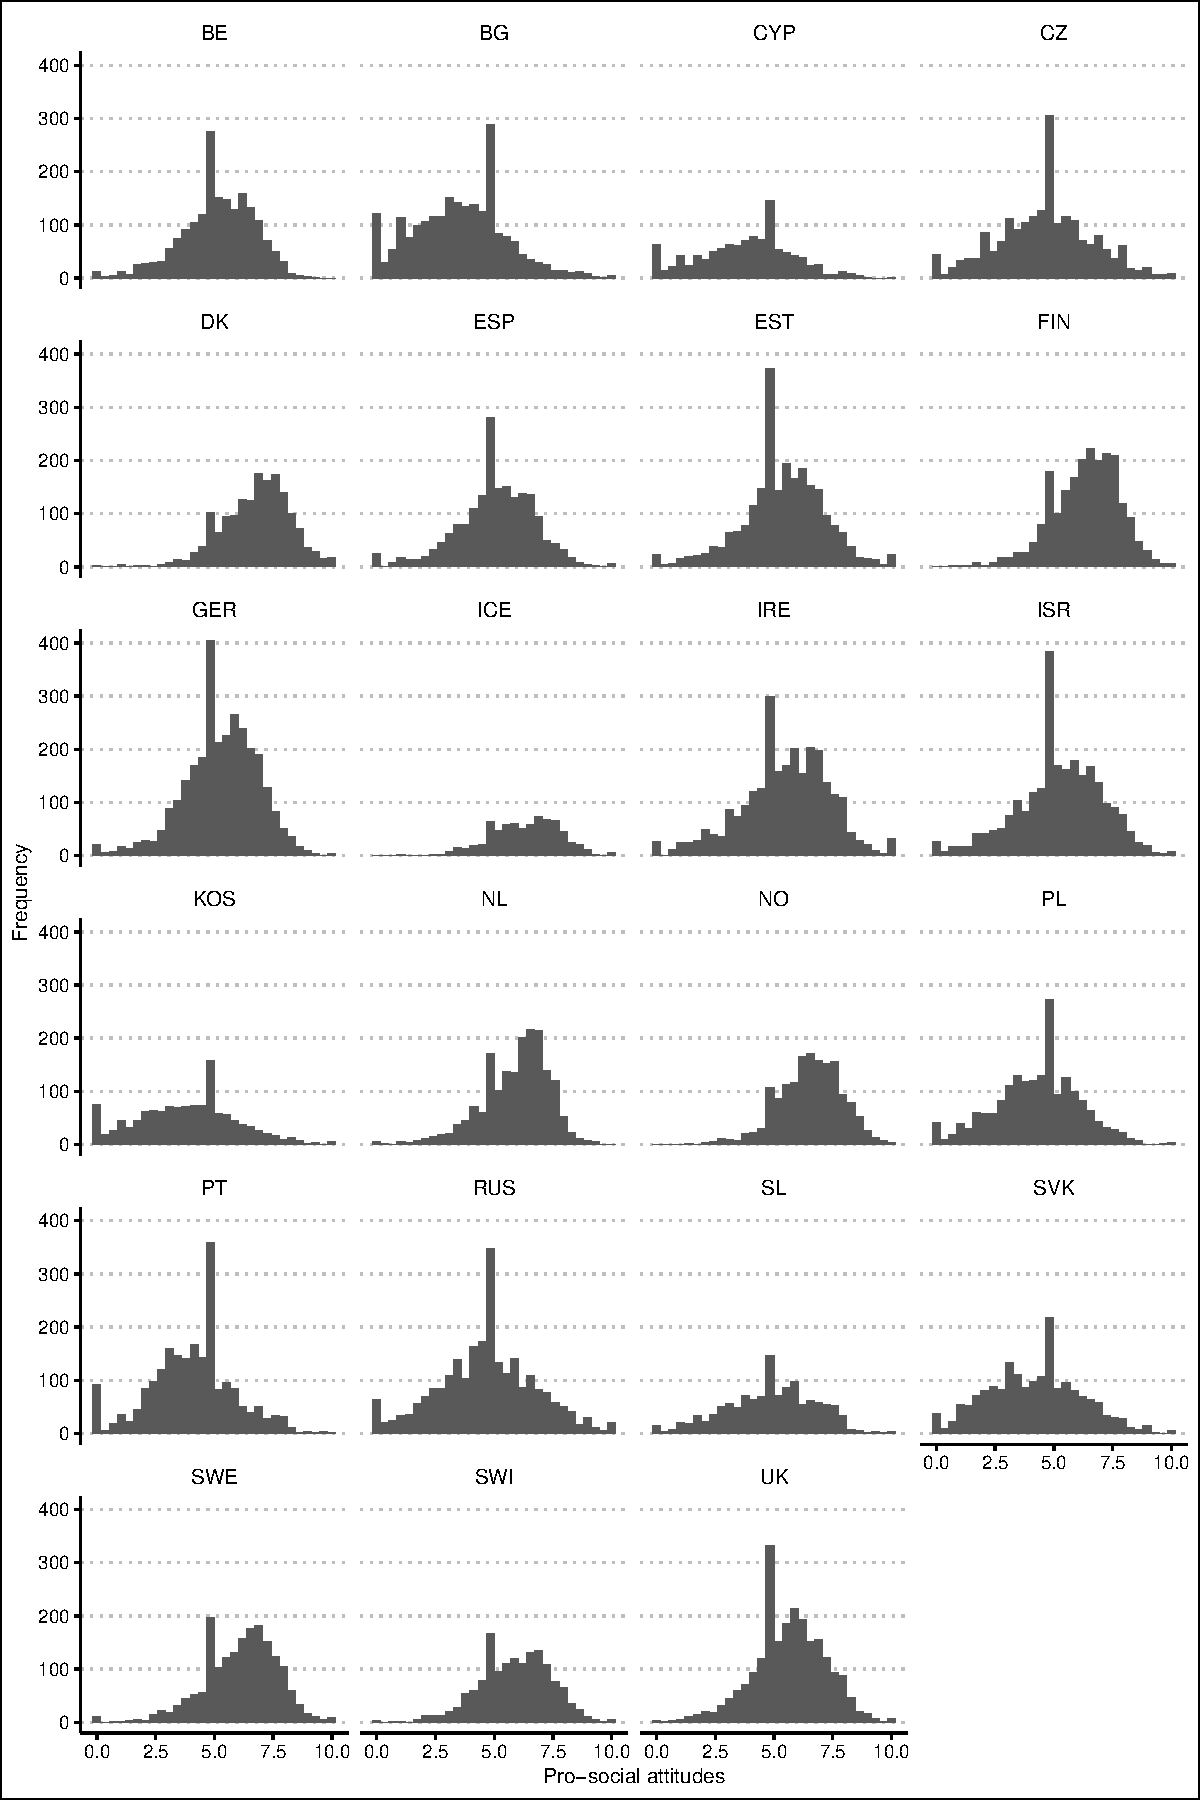
\includegraphics[scale=0.75]{../../05-graphs/Supplem-03.pdf}
 \caption{\label{fig:fig-01} Distribution of pro-social attitudes per country}
\end{figure}

As can be quickly seen from Figure~\ref{fig:fig-01} on page~\pageref{fig:fig-01}, the distribution of the dependent variable is roughly normal in almost all countries in the sample. The only problem is the unexpectedly large number of answers of ``5'' on the scale for most countries. These are producing the spikes clearly seen in most panels of Figure~\ref{fig:fig-01}. As there is not much that can be done to correct this problem, we are left with no choice but to proceed with the analysis.

\afterpage{\clearpage}

\section{Analyses}
At the individual level, I will be interested in the relationship between education and pro-social attitudes. At the contextual level, I am keen on exploring how corruption impacts these same attitudes. To begin with, let's see whether there is any effect between education and pro-social attitudes, the shape of this effect, and whether it varies between national contexts.

\begin{knitrout}
\definecolor{shadecolor}{rgb}{0.969, 0.969, 0.969}\color{fgcolor}\begin{kframe}
\begin{alltt}
\hlkwd{ggplot}\hlstd{(}\hlkwc{data} \hlstd{= df_ess,}
       \hlkwd{aes}\hlstd{(}\hlkwc{x} \hlstd{= eduyrs,} \hlkwc{y} \hlstd{= trustind))} \hlopt{+}
  \hlkwd{facet_wrap}\hlstd{(}\hlopt{~} \hlstd{cntry,} \hlkwc{ncol} \hlstd{=} \hlnum{4}\hlstd{)} \hlopt{+}
  \hlkwd{stat_density_2d}\hlstd{()} \hlopt{+}
  \hlkwd{geom_smooth}\hlstd{(}\hlkwc{method} \hlstd{=} \hlstr{"lm"}\hlstd{,}
              \hlkwc{se}\hlstd{=}\hlnum{FALSE}\hlstd{,}
              \hlkwc{color} \hlstd{=} \hlstr{"red"}\hlstd{,}
              \hlkwc{linewidth} \hlstd{=} \hlnum{1.5}\hlstd{)} \hlopt{+}
  \hlkwd{theme_clean}\hlstd{()} \hlopt{+}
  \hlkwd{labs}\hlstd{(}\hlkwc{x} \hlstd{=} \hlstr{"Years of education"}\hlstd{,}
       \hlkwc{y} \hlstd{=} \hlstr{"Pro-social attitudes"}\hlstd{)}
\end{alltt}
\end{kframe}
\end{knitrout}



The plot can be seen in Figure~\ref{fig:fig-02} on page \pageref{fig:fig-02} and presents us with considerable insights. To begin with, there is some variation in the relationship between education and pro-social attitudes. In some countries the relationship is clearly positive (BG, GER, SWE), while in others there appears to be no relationship (FIN, CZ, RUS). Finally, there is also the extreme case of Kosovo, where the relationship is negative.\footnote{If this were an actual analysis, this is the stage where some deep thought would be put into whether Kosovo should be kept in the sample if it exhibits this unusual relationship. In my demo analysis I don't have to worry very much, as Kosovo will drop out of the sample due to missing information on the CPI and Gini index.} More stories surface though. We can see from where the highest density of points is located that countries exhibit different average levels of pro-social attitudes. A clear distinction can be made between post-communist countries, at one end, and Scandinavian nations at the other end. The easiest spot in Figure~\ref{fig:fig-02} where this can be seen is the row that contains Kosovo, Norway and Poland, almost side by side. We see, then, that a post-communism dummy should likely be added to the analysis.

\begin{figure}[!ht]
  \centering
  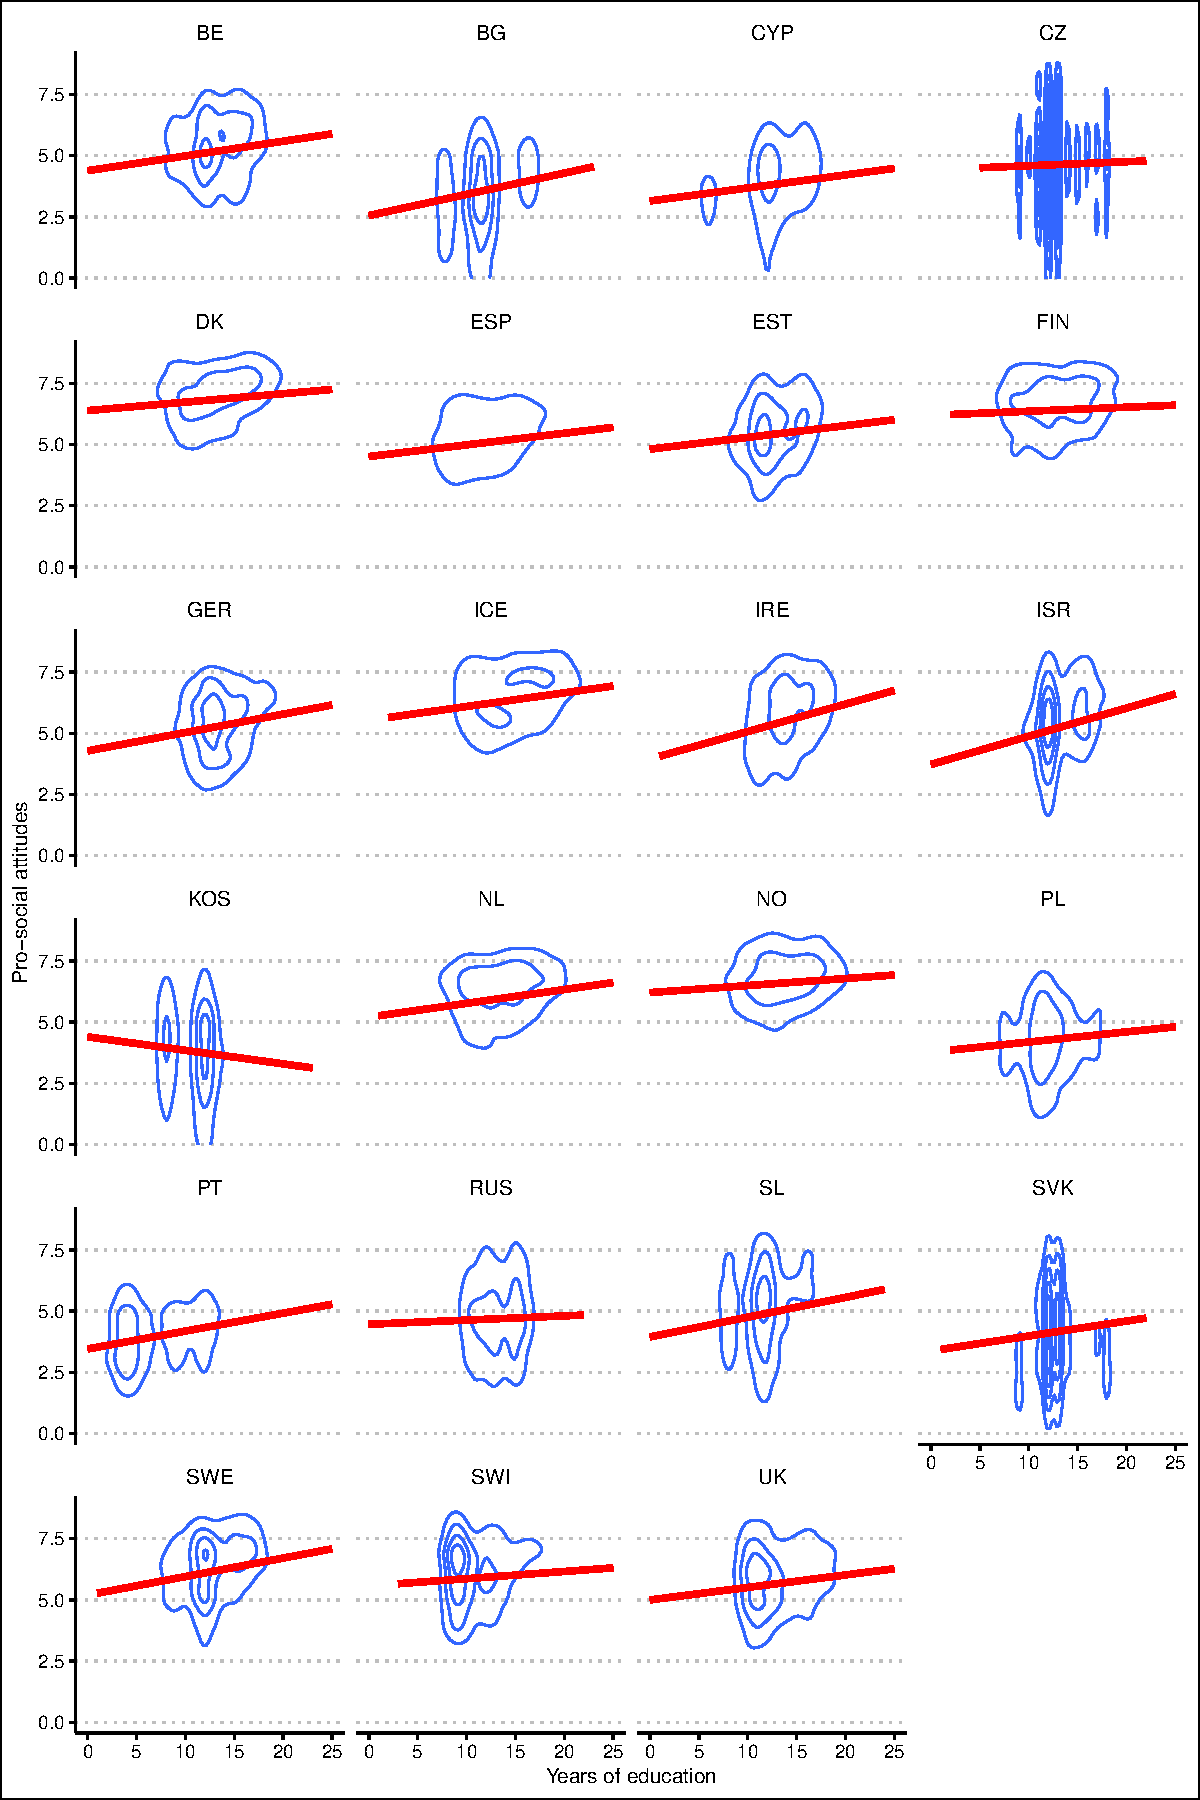
\includegraphics[scale=0.75]{../../05-graphs/Supplem-04}
  \caption{\label{fig:fig-02} Relationship between education and pro-social attitudes}
\end{figure}

To begin with, let's run a simple null model---without any substantive predictors in the model. Before this, though, I have to center and standardize the variables I will be using in the analysis, and then clear all missing values.

\begin{knitrout}
\definecolor{shadecolor}{rgb}{0.969, 0.969, 0.969}\color{fgcolor}\begin{kframe}
\begin{alltt}
\hlcom{# Group-mean centering}
\hlstd{df_ess} \hlopt
  \hlkwd{group_by}\hlstd{(cntry)} \hlopt
  \hlkwd{mutate}\hlstd{(}\hlkwc{age.cwc} \hlstd{= arm}\hlopt{::}\hlkwd{rescale}\hlstd{(agea),}
         \hlkwc{gend.cwc} \hlstd{= arm}\hlopt{::}\hlkwd{rescale}\hlstd{(male),}
         \hlkwc{edu.cwc} \hlstd{= arm}\hlopt{::}\hlkwd{rescale}\hlstd{(eduyrs),}
         \hlkwc{inc.cwc} \hlstd{= arm}\hlopt{::}\hlkwd{rescale}\hlstd{(hinctnta))}

\hlcom{# Create country-level data}
\hlstd{df_agg} \hlkwb{<-} \hlstd{df_ess} \hlopt
  \hlkwd{group_by}\hlstd{(cntry)} \hlopt
  \hlkwd{distinct}\hlstd{(gini_net, ti_cpi, postcom)} \hlopt
  \hlkwd{as.data.frame}\hlstd{()}

\hlstd{df_agg} \hlopt
  \hlkwd{mutate}\hlstd{(}\hlkwc{gini.cgm} \hlstd{= arm}\hlopt{::}\hlkwd{rescale}\hlstd{(gini_net),}
         \hlkwc{postcom.cgm} \hlstd{= arm}\hlopt{::}\hlkwd{rescale}\hlstd{(postcom),}
         \hlkwc{cpi.cgm} \hlstd{= arm}\hlopt{::}\hlkwd{rescale}\hlstd{(ti_cpi))} \hlopt
  \hlstd{dplyr}\hlopt{::}\hlkwd{select}\hlstd{(}\hlopt{-}\hlkwd{c}\hlstd{(gini_net, ti_cpi, postcom))}

\hlstd{df_ess} \hlkwb{<-} \hlkwd{left_join}\hlstd{(df_ess, df_agg,} \hlkwc{by} \hlstd{=} \hlkwd{c}\hlstd{(}\hlstr{"cntry"}\hlstd{))}
\hlkwd{rm}\hlstd{(df_agg)}

\hlcom{# Select only variables used and do listwise deletion}
\hlstd{df_sub} \hlkwb{<-} \hlstd{df_ess} \hlopt
  \hlstd{dplyr}\hlopt{::}\hlkwd{select}\hlstd{(cntry, age.cwc, gend.cwc, edu.cwc, inc.cwc,}
                \hlstd{gini.cgm, postcom.cgm, cpi.cgm, trustind)} \hlopt
  \hlkwd{na.omit}\hlstd{()}

\hlstd{model0} \hlkwb{<-} \hlkwd{lmer}\hlstd{(trustind} \hlopt{~} \hlnum{1} \hlopt{+} \hlstd{(}\hlnum{1} \hlopt{|} \hlstd{cntry),} \hlcom{# Specify model}
               \hlkwc{data} \hlstd{= df_sub,} \hlcom{# Data to estimate model on}
               \hlkwc{na.action} \hlstd{= na.omit,} \hlcom{# Ignore missing cases}
               \hlkwc{REML} \hlstd{=} \hlnum{TRUE}\hlstd{)} \hlcom{# REML estimation for parameters}
\hlkwd{summary}\hlstd{(model0)}
\end{alltt}
\begin{verbatim}
Linear mixed model fit by REML ['lmerMod']
Formula: trustind ~ 1 + (1 | cntry)
   Data: df_sub

REML criterion at convergence: 125382.3

Scaled residuals: 
    Min      1Q  Median      3Q     Max 
-3.9242 -0.6198  0.0740  0.6961  3.6769 

Random effects:
 Groups   Name        Variance Std.Dev.
 cntry    (Intercept) 0.9326   0.9657  
 Residual             3.0644   1.7505  
Number of obs: 31648, groups:  cntry, 21

Fixed effects:
            Estimate Std. Error t value
(Intercept)    5.270      0.211   24.98
\end{verbatim}
\end{kframe}
\end{knitrout}

The model is estimated with REML, with individuals nested in countries. The ICC is the ratio of country intercept residual variance and total variance: $\frac{0.9326}{0.9326+3.0644}$= 0.233325. You can extract any needed quantities from the model, starting with fixed effects, random effects, SEs for fixed effects and random effects using the \texttt{fixef()}, \texttt{ranef()}, \texttt{se.fixef()} or \texttt{se.ranef()} functions from the \texttt{arm} package.

\begin{knitrout}
\definecolor{shadecolor}{rgb}{0.969, 0.969, 0.969}\color{fgcolor}\begin{kframe}
\begin{alltt}
\hlkwd{fixef}\hlstd{(model0)}
\hlkwd{se.fixef}\hlstd{(model0)}
\end{alltt}
\end{kframe}
\end{knitrout}

\begin{knitrout}
\definecolor{shadecolor}{rgb}{0.969, 0.969, 0.969}\color{fgcolor}\begin{kframe}
\begin{alltt}
\hlkwd{ranef}\hlstd{(model0)}
\hlkwd{se.ranef}\hlstd{(model0)}
\end{alltt}
\end{kframe}
\end{knitrout}

\begin{table}[!h]

\caption{\label{tab:ch-8}First 10 random effects}
\centering
\begin{tabular}[t]{lrr}
\toprule
Country & RE & SE\\
\midrule
BE & -0.1101089 & 0.0431440\\
BG & -1.7068509 & 0.0397616\\
CYP & -1.4605981 & 0.0590348\\
CZ & -0.6583279 & 0.0475859\\
DK & 1.5991362 & 0.0473416\\
ESP & -0.1883927 & 0.0452247\\
EST & 0.1395813 & 0.0400206\\
FIN & 1.1443538 & 0.0391797\\
GER & 0.0471130 & 0.0351994\\
ICE & 1.1233698 & 0.0713299\\
\bottomrule
\end{tabular}
\end{table}



Keep in mind that these are not actual values of trust for each country; they are \textit{deviations} of the countries from the overall level of trust. This is why some of them are negative, wile others are positive. You can also get a few model fit criteria with a few basic functions.

\begin{knitrout}
\definecolor{shadecolor}{rgb}{0.969, 0.969, 0.969}\color{fgcolor}\begin{kframe}
\begin{alltt}
\hlkwd{AIC}\hlstd{(model0)}
\end{alltt}
\begin{verbatim}
[1] 125388.3
\end{verbatim}
\begin{alltt}
\hlkwd{BIC}\hlstd{(model0)}
\end{alltt}
\begin{verbatim}
[1] 125413.3
\end{verbatim}
\begin{alltt}
\hlkwd{logLik}\hlstd{(model0)}
\end{alltt}
\begin{verbatim}
'log Lik.' -62691.13 (df=3)
\end{verbatim}
\end{kframe}
\end{knitrout}

My advice in terms of mixed-effects modeling is to start from simple models and gradually build up the model complexity. That way, if there are estimation warnings or errors, you can quickly diagnose which was the ``guilty'' predictor. If you start off from very complex specifications, it will be very difficult to figure out which of a number of fixed effects or random effects is the culprit. Here, I've started first with the individual-level predictors of pro-social attitudes.

\begin{knitrout}
\definecolor{shadecolor}{rgb}{0.969, 0.969, 0.969}\color{fgcolor}\begin{kframe}
\begin{alltt}
\hlstd{model1} \hlkwb{<-} \hlkwd{lmer}\hlstd{(trustind} \hlopt{~} \hlstd{age.cwc} \hlopt{+} \hlstd{gend.cwc} \hlopt{+} \hlstd{edu.cwc} \hlopt{+}
                 \hlstd{inc.cwc} \hlopt{+} \hlstd{(}\hlnum{1} \hlopt{|} \hlstd{cntry),}
               \hlkwc{data} \hlstd{= df_sub,}
               \hlkwc{REML} \hlstd{=} \hlnum{TRUE}\hlstd{)}
\hlkwd{summary}\hlstd{(model1)}
\end{alltt}
\begin{verbatim}
Linear mixed model fit by REML ['lmerMod']
Formula: trustind ~ age.cwc + gend.cwc + edu.cwc + inc.cwc + (1 | cntry)
   Data: df_sub

REML criterion at convergence: 124411.3

Scaled residuals: 
    Min      1Q  Median      3Q     Max 
-4.1698 -0.6249  0.0651  0.6674  3.9275 

Random effects:
 Groups   Name        Variance Std.Dev.
 cntry    (Intercept) 0.9263   0.9625  
 Residual             2.9699   1.7233  
Number of obs: 31648, groups:  cntry, 21

Fixed effects:
            Estimate Std. Error t value
(Intercept)  5.26370    0.21028  25.032
age.cwc      0.29995    0.02092  14.335
gend.cwc    -0.13135    0.01961  -6.697
edu.cwc      0.38010    0.02148  17.698
inc.cwc      0.38925    0.02116  18.399

Correlation of Fixed Effects:
         (Intr) ag.cwc gnd.cw ed.cwc
age.cwc  -0.002                     
gend.cwc  0.000  0.017              
edu.cwc  -0.002  0.242  0.030       
inc.cwc   0.001  0.128 -0.100 -0.323
\end{verbatim}
\end{kframe}
\end{knitrout}

The results are consistent with what we would expect. A 2 SD increase in age would lead to a 0.3 increase in the level of pro-social attitudes, measured on a 0--10 scale. Men appear to be about -0.13 points less pro-social than women, on average. Both education and income have positive and statistically significant effects on the extent to which an individual exhibits pro-social attitudes. While the null model has an AIC of \ensuremath{1.2538825\times 10^{5}} and a logLikelihood of \ensuremath{-6.269113\times 10^{4}}, the AIC of the model with only individual-level predictors is \ensuremath{1.2442526\times 10^{5}}, and the logLikelihood is \ensuremath{-6.220563\times 10^{4}}. With this difference between logLikelihoods there is little reason for a likelihood ratio test: the second model fits the data much better than the first one.\footnote{Remember, larger value for the logLikelihood denote a better fitting model. On the negative scale numbers that are closer to 0 are considered larger than numbers that are farther away from 0.}

We  can now proceed to running a model with both individual-level and country-level predictors of pro-social attitudes.

\begin{knitrout}
\definecolor{shadecolor}{rgb}{0.969, 0.969, 0.969}\color{fgcolor}\begin{kframe}
\begin{alltt}
\hlstd{model2} \hlkwb{<-} \hlkwd{lmer}\hlstd{(trustind} \hlopt{~} \hlstd{age.cwc} \hlopt{+} \hlstd{gend.cwc} \hlopt{+} \hlstd{edu.cwc} \hlopt{+}
                 \hlstd{inc.cwc} \hlopt{+} \hlstd{gini.cgm} \hlopt{+} \hlstd{postcom.cgm} \hlopt{+} \hlstd{cpi.cgm} \hlopt{+}
                 \hlstd{(}\hlnum{1} \hlopt{|} \hlstd{cntry),}
               \hlkwc{data} \hlstd{= df_sub,}
               \hlkwc{REML} \hlstd{=} \hlnum{TRUE}\hlstd{)}
\hlkwd{summary}\hlstd{(model2)}
\end{alltt}
\begin{verbatim}
Linear mixed model fit by REML ['lmerMod']
Formula: trustind ~ age.cwc + gend.cwc + edu.cwc + inc.cwc + gini.cgm +  
    postcom.cgm + cpi.cgm + (1 | cntry)
   Data: df_sub

REML criterion at convergence: 124384.2

Scaled residuals: 
    Min      1Q  Median      3Q     Max 
-4.1688 -0.6255  0.0648  0.6668  3.9278 

Random effects:
 Groups   Name        Variance Std.Dev.
 cntry    (Intercept) 0.2531   0.5031  
 Residual             2.9699   1.7233  
Number of obs: 31648, groups:  cntry, 21

Fixed effects:
            Estimate Std. Error t value
(Intercept)  5.24718    0.11032  47.564
age.cwc      0.29991    0.02092  14.333
gend.cwc    -0.13138    0.01961  -6.699
edu.cwc      0.38006    0.02148  17.696
inc.cwc      0.38923    0.02116  18.398
gini.cgm     0.35080    0.29519   1.188
postcom.cgm  0.84480    0.43352   1.949
cpi.cgm      2.42905    0.47644   5.098

Correlation of Fixed Effects:
            (Intr) ag.cwc gnd.cw ed.cwc inc.cw gn.cgm pstcm.
age.cwc     -0.003                                          
gend.cwc    -0.001  0.017                                   
edu.cwc     -0.003  0.242  0.030                            
inc.cwc      0.001  0.128 -0.100 -0.323                     
gini.cgm    -0.010  0.000  0.000  0.000  0.000              
postcom.cgm  0.014 -0.001  0.000 -0.002  0.000  0.408       
cpi.cgm     -0.005  0.000  0.000 -0.003  0.001  0.616  0.832
\end{verbatim}
\end{kframe}
\end{knitrout}

Neither the effect of Gini or the post-communism dummy are statistically significant. However, in the case of post-communism, the effect is fairly strong which suggests that there might be something there. It's possible that this is a legacy of the Communist past, or something related to the cutthroat competitive environment immediately following the fall of Communism. On the other hand, the effect of corruption perceptions is clearly positive and statistically significant. A 2 SD increase in CPI (roughly speaking, 4.1 points on a 11 point scale, or about the difference between Romania and Norway in 2013) is associated with an average increase in pro-social attitudes of 2.43 points.\footnote{The CPI is reverse coded: increases in the score denote less corruption.} Does this new model fit the data better than the previous one, though?

\begin{knitrout}
\definecolor{shadecolor}{rgb}{0.969, 0.969, 0.969}\color{fgcolor}\begin{kframe}
\begin{alltt}
\hlkwd{anova}\hlstd{(model1, model2)}
\end{alltt}
\begin{verbatim}
Data: df_sub
Models:
model1: trustind ~ age.cwc + gend.cwc + edu.cwc + inc.cwc + (1 | cntry)
model2: trustind ~ age.cwc + gend.cwc + edu.cwc + inc.cwc + gini.cgm + postcom.cgm + cpi.cgm + (1 | cntry)
       npar    AIC    BIC logLik deviance  Chisq Df Pr(>Chisq)    
model1    7 124400 124459 -62193   124386                         
model2   10 124376 124459 -62178   124356 30.509  3  1.079e-06 ***
---
Signif. codes:  0 '***' 0.001 '**' 0.01 '*' 0.05 '.' 0.1 ' ' 1
\end{verbatim}
\end{kframe}
\end{knitrout}

The likelihood ratio test can be used to compare the fit of the two models, to determine which is the better fitting model. There is a version of the test in the \texttt{lmtest} package, with the \texttt{lrtest()} command, but I suggest the standard \texttt{anova()} function. This has the benefit of correcting any user mistakes---if two models that differ in their fixed components are estimated with REML and then compared, \texttt{anova()} will re-estimate the models with FIML. With 10 estimated parameters (8 fixed effects and 2 random effects), Model 2 is shown to fit the data better than Model 1.

\begin{knitrout}
\definecolor{shadecolor}{rgb}{0.969, 0.969, 0.969}\color{fgcolor}\begin{kframe}
\begin{alltt}
\hlstd{model3} \hlkwb{<-} \hlkwd{lmer}\hlstd{(trustind} \hlopt{~} \hlstd{age.cwc} \hlopt{+} \hlstd{gend.cwc} \hlopt{+} \hlstd{edu.cwc} \hlopt{+}
                 \hlstd{inc.cwc} \hlopt{+} \hlstd{gini.cgm} \hlopt{+} \hlstd{postcom.cgm} \hlopt{+} \hlstd{cpi.cgm} \hlopt{+}
                 \hlstd{(}\hlnum{1} \hlopt{+} \hlstd{edu.cwc} \hlopt{|} \hlstd{cntry),}
               \hlkwc{data} \hlstd{= df_sub,}
               \hlkwc{REML} \hlstd{=} \hlnum{TRUE}\hlstd{)}
\hlkwd{summary}\hlstd{(model3)}
\end{alltt}
\begin{verbatim}
Linear mixed model fit by REML ['lmerMod']
Formula: trustind ~ age.cwc + gend.cwc + edu.cwc + inc.cwc + gini.cgm +  
    postcom.cgm + cpi.cgm + (1 + edu.cwc | cntry)
   Data: df_sub

REML criterion at convergence: 124325.8

Scaled residuals: 
    Min      1Q  Median      3Q     Max 
-4.0568 -0.6222  0.0655  0.6676  3.9546 

Random effects:
 Groups   Name        Variance Std.Dev. Corr 
 cntry    (Intercept) 0.2503   0.5003        
          edu.cwc     0.0336   0.1833   -0.61
 Residual             2.9619   1.7210        
Number of obs: 31648, groups:  cntry, 21

Fixed effects:
            Estimate Std. Error t value
(Intercept)  5.24721    0.10969  47.836
age.cwc      0.30639    0.02100  14.591
gend.cwc    -0.13358    0.01961  -6.812
edu.cwc      0.38774    0.04571   8.483
inc.cwc      0.38352    0.02117  18.119
gini.cgm     0.23670    0.24644   0.960
postcom.cgm  0.46086    0.36330   1.269
cpi.cgm      2.10215    0.39875   5.272

Correlation of Fixed Effects:
            (Intr) ag.cwc gnd.cw ed.cwc inc.cw gn.cgm pstcm.
age.cwc     -0.003                                          
gend.cwc    -0.001  0.018                                   
edu.cwc     -0.531  0.116  0.013                            
inc.cwc      0.001  0.125 -0.100 -0.152                     
gini.cgm    -0.009  0.001  0.004 -0.020 -0.004              
postcom.cgm  0.011 -0.012  0.004 -0.014  0.002  0.403       
cpi.cgm     -0.005 -0.010  0.004 -0.019  0.005  0.616  0.832
\end{verbatim}
\end{kframe}
\end{knitrout}

Does Model 3 fit the data better than Model 2? To rephrase it in a clearer way, do we have any reason to believe that the slope of education varies across countries?

\begin{knitrout}
\definecolor{shadecolor}{rgb}{0.969, 0.969, 0.969}\color{fgcolor}\begin{kframe}
\begin{alltt}
\hlkwd{anova}\hlstd{(model2, model3)}
\end{alltt}
\begin{verbatim}
Data: df_sub
Models:
model2: trustind ~ age.cwc + gend.cwc + edu.cwc + inc.cwc + gini.cgm + postcom.cgm + cpi.cgm + (1 | cntry)
model3: trustind ~ age.cwc + gend.cwc + edu.cwc + inc.cwc + gini.cgm + postcom.cgm + cpi.cgm + (1 + edu.cwc | cntry)
       npar    AIC    BIC logLik deviance  Chisq Df Pr(>Chisq)    
model2   10 124376 124459 -62178   124356                         
model3   12 124321 124422 -62149   124297 58.186  2  2.318e-13 ***
---
Signif. codes:  0 '***' 0.001 '**' 0.01 '*' 0.05 '.' 0.1 ' ' 1
\end{verbatim}
\end{kframe}
\end{knitrout}

The results again suggest that the more complex model fits the data better. Adding two parameters to the estimation procedure (an extra random effect and the correlation between random effects) produced a significantly better fit to the data, as indicated by the likelihood ratio test we ran above. Finally, we can test to see whether corruption perceptions are a predictor of the relationship between education and pro-social attitudes

\begin{knitrout}
\definecolor{shadecolor}{rgb}{0.969, 0.969, 0.969}\color{fgcolor}\begin{kframe}
\begin{alltt}
\hlstd{model4} \hlkwb{<-} \hlkwd{lmer}\hlstd{(trustind} \hlopt{~} \hlstd{age.cwc} \hlopt{+} \hlstd{gend.cwc} \hlopt{+} \hlstd{edu.cwc} \hlopt{+}
                 \hlstd{inc.cwc} \hlopt{+} \hlstd{gini.cgm} \hlopt{+} \hlstd{postcom.cgm} \hlopt{+} \hlstd{cpi.cgm} \hlopt{+}
                 \hlstd{edu.cwc}\hlopt{*}\hlstd{cpi.cgm} \hlopt{+} \hlstd{(}\hlnum{1} \hlopt{+} \hlstd{edu.cwc} \hlopt{|} \hlstd{cntry),}
               \hlkwc{data} \hlstd{= df_sub,}
               \hlkwc{control}\hlstd{=}\hlkwd{lmerControl}\hlstd{(}\hlkwc{optCtrl} \hlstd{=} \hlkwd{list}\hlstd{(}\hlkwc{maxfun}\hlstd{=}\hlnum{100000}\hlstd{),}
                                   \hlkwc{optimizer} \hlstd{=} \hlstr{"bobyqa"}\hlstd{),}
               \hlkwc{REML} \hlstd{=} \hlnum{TRUE}\hlstd{)}
\hlkwd{summary}\hlstd{(model4)}
\end{alltt}
\begin{verbatim}
Linear mixed model fit by REML ['lmerMod']
Formula: trustind ~ age.cwc + gend.cwc + edu.cwc + inc.cwc + gini.cgm +  
    postcom.cgm + cpi.cgm + edu.cwc * cpi.cgm + (1 + edu.cwc |      cntry)
   Data: df_sub
Control: lmerControl(optCtrl = list(maxfun = 1e+05), optimizer = "bobyqa")

REML criterion at convergence: 124328.8

Scaled residuals: 
    Min      1Q  Median      3Q     Max 
-4.0567 -0.6216  0.0651  0.6674  3.9541 

Random effects:
 Groups   Name        Variance Std.Dev. Corr 
 cntry    (Intercept) 0.25401  0.5040        
          edu.cwc     0.03569  0.1889   -0.61
 Residual             2.96194  1.7210        
Number of obs: 31648, groups:  cntry, 21

Fixed effects:
                Estimate Std. Error t value
(Intercept)      5.24751    0.11050  47.488
age.cwc          0.30645    0.02100  14.592
gend.cwc        -0.13359    0.01961  -6.813
edu.cwc          0.38760    0.04681   8.280
inc.cwc          0.38351    0.02117  18.117
gini.cgm         0.23775    0.24654   0.964
postcom.cgm      0.46121    0.36342   1.269
cpi.cgm          2.07654    0.41688   4.981
edu.cwc:cpi.cgm  0.01937    0.09146   0.212

Correlation of Fixed Effects:
            (Intr) ag.cwc gnd.cw ed.cwc inc.cw gn.cgm pstcm. cp.cgm
age.cwc     -0.003                                                 
gend.cwc    -0.001  0.018                                          
edu.cwc     -0.540  0.114  0.013                                   
inc.cwc      0.001  0.124 -0.100 -0.149                            
gini.cgm    -0.008  0.001  0.004 -0.020 -0.004                     
postcom.cgm  0.011 -0.012  0.004 -0.014  0.002  0.403              
cpi.cgm     -0.008 -0.007  0.003 -0.010  0.001  0.586  0.795       
ed.cwc:cp.c  0.012 -0.007  0.001 -0.028  0.015  0.012  0.002 -0.291
\end{verbatim}
\end{kframe}
\end{knitrout}

Unfortunately, the model output indicates that corruption perceptions are not a moderator of the relationship between education and pro-social attitudes.\footnote{I increased the maximum number of iterations, as well as changed the optimizer to \texttt{bobyqa} (``bound optimization by quadratic approximation'').} The coefficient for the interaction term is as far away from statistical significance as it can get. This is also indicated by the comparison of model fit statistics, which gives us little reason to increase the complexity of the model: the more intricate model does not fit the data significantly better than the less complex one.

\begin{knitrout}
\definecolor{shadecolor}{rgb}{0.969, 0.969, 0.969}\color{fgcolor}\begin{kframe}
\begin{alltt}
\hlkwd{anova}\hlstd{(model3, model4)}
\end{alltt}
\begin{verbatim}
Data: df_sub
Models:
model3: trustind ~ age.cwc + gend.cwc + edu.cwc + inc.cwc + gini.cgm + postcom.cgm + cpi.cgm + (1 + edu.cwc | cntry)
model4: trustind ~ age.cwc + gend.cwc + edu.cwc + inc.cwc + gini.cgm + postcom.cgm + cpi.cgm + edu.cwc * cpi.cgm + (1 + edu.cwc | cntry)
       npar    AIC    BIC logLik deviance Chisq Df Pr(>Chisq)
model3   12 124321 124422 -62149   124297                    
model4   13 124323 124432 -62149   124297 0.046  1     0.8302
\end{verbatim}
\begin{alltt}
\hlcom{# Clearly, model 4 does not fit the data better than}
\hlcom{#   model 3.}
\end{alltt}
\end{kframe}
\end{knitrout}


\section{Displaying model results}

A standard way of presenting model results are regression comparison tables, easily generated through the \texttt{apsrtable}, \texttt{stargazer}, or \texttt{texreg} packages for R. In this example, I will use the latter package.

\begin{kframe}
\begin{alltt}
\hlcom{# For LaTeX output}
\hlkwd{texreg}\hlstd{(}\hlkwd{list}\hlstd{(model0, model1, model2, model3, model4),}
       \hlkwc{digits}\hlstd{=}\hlnum{2}\hlstd{,}
       \hlkwc{custom.model.names}\hlstd{=}\hlkwd{c}\hlstd{(}\hlstr{"Null model"}\hlstd{,} \hlstr{"Model 1"}\hlstd{,} \hlstr{"Model 2"}\hlstd{,}
                            \hlstr{"Model 3"}\hlstd{,} \hlstr{"Model 4"}\hlstd{),}
       \hlkwc{custom.coef.names}\hlstd{=}\hlkwd{c}\hlstd{(}\hlstr{"(Intercept)"}\hlstd{,} \hlstr{"Age (decades)"}\hlstd{,}
                           \hlstr{"Male"}\hlstd{,} \hlstr{"Education"}\hlstd{,} \hlstr{"Income"}\hlstd{,}
                           \hlstr{"Gini"}\hlstd{,} \hlstr{"Post-communism"}\hlstd{,}
                           \hlstr{"CPI index"}\hlstd{,}\hlstr{"Education*CPI"}\hlstd{))}
\hlcom{# For HTML output, that can be read into Word}
\hlkwd{htmlreg}\hlstd{(}\hlkwd{list}\hlstd{(model0, model1, model2, model3, model4),}
        \hlkwc{digits}\hlstd{=}\hlnum{2}\hlstd{,}
        \hlkwc{custom.model.names}\hlstd{=}\hlkwd{c}\hlstd{(}\hlstr{"Null model"}\hlstd{,} \hlstr{"Model 1"}\hlstd{,} \hlstr{"Model 2"}\hlstd{,}
                             \hlstr{"Model 3"}\hlstd{,} \hlstr{"Model 4"}\hlstd{),}
        \hlkwc{custom.coef.names}\hlstd{=}\hlkwd{c}\hlstd{(}\hlstr{"(Intercept)"}\hlstd{,} \hlstr{"Age (decades)"}\hlstd{,}
                            \hlstr{"Male"}\hlstd{,} \hlstr{"Education"}\hlstd{,} \hlstr{"Income"}\hlstd{,}
                            \hlstr{"Gini"}\hlstd{,} \hlstr{"Post-communism"}\hlstd{,}
                            \hlstr{"CPI index"}\hlstd{,}\hlstr{"Education*CPI"}\hlstd{))}
\hlcom{# For output displayed in your R console}
\hlkwd{screenreg}\hlstd{(}\hlkwd{list}\hlstd{(model0, model1, model2, model3, model4),}
          \hlkwc{digits}\hlstd{=}\hlnum{2}\hlstd{,}
          \hlkwc{custom.model.names}\hlstd{=}\hlkwd{c}\hlstd{(}\hlstr{"Null model"}\hlstd{,} \hlstr{"Model 1"}\hlstd{,} \hlstr{"Model 2"}\hlstd{,}
                               \hlstr{"Model 3"}\hlstd{,} \hlstr{"Model 4"}\hlstd{),}
          \hlkwc{custom.coef.names}\hlstd{=}\hlkwd{c}\hlstd{(}\hlstr{"(Intercept)"}\hlstd{,} \hlstr{"Age (decades)"}\hlstd{,}
                              \hlstr{"Male"}\hlstd{,} \hlstr{"Education"}\hlstd{,} \hlstr{"Income"}\hlstd{,}
                              \hlstr{"Gini"}\hlstd{,} \hlstr{"Post-communism"}\hlstd{,}
                              \hlstr{"CPI index"}\hlstd{,}\hlstr{"Education*CPI"}\hlstd{))}
\end{alltt}
\end{kframe}


\begin{table}[!ht]
\caption{Statistical models}
\begin{center}
\begin{footnotesize}
\begin{tabular}{l D{.}{.}{6.5} D{.}{.}{6.5} D{.}{.}{6.5} D{.}{.}{6.5} D{.}{.}{6.5}}
\toprule
 & \multicolumn{1}{c}{Null model} & \multicolumn{1}{c}{Model 1} & \multicolumn{1}{c}{Model 2} & \multicolumn{1}{c}{Model 3} & \multicolumn{1}{c}{Model 4} \\
\midrule
(Intercept)                    & 5.27^{***} & 5.26^{***}  & 5.25^{***}  & 5.25^{***}  & 5.25^{***}  \\
                               & (0.21)     & (0.21)      & (0.11)      & (0.11)      & (0.11)      \\
Age (decades)                  &            & 0.30^{***}  & 0.30^{***}  & 0.31^{***}  & 0.31^{***}  \\
                               &            & (0.02)      & (0.02)      & (0.02)      & (0.02)      \\
Male                           &            & -0.13^{***} & -0.13^{***} & -0.13^{***} & -0.13^{***} \\
                               &            & (0.02)      & (0.02)      & (0.02)      & (0.02)      \\
Education                      &            & 0.38^{***}  & 0.38^{***}  & 0.39^{***}  & 0.39^{***}  \\
                               &            & (0.02)      & (0.02)      & (0.05)      & (0.05)      \\
Income                         &            & 0.39^{***}  & 0.39^{***}  & 0.38^{***}  & 0.38^{***}  \\
                               &            & (0.02)      & (0.02)      & (0.02)      & (0.02)      \\
Gini                           &            &             & 0.35        & 0.24        & 0.24        \\
                               &            &             & (0.30)      & (0.25)      & (0.25)      \\
Post-communism                 &            &             & 0.84        & 0.46        & 0.46        \\
                               &            &             & (0.43)      & (0.36)      & (0.36)      \\
CPI index                      &            &             & 2.43^{***}  & 2.10^{***}  & 2.08^{***}  \\
                               &            &             & (0.48)      & (0.40)      & (0.42)      \\
Education*CPI                  &            &             &             &             & 0.02        \\
                               &            &             &             &             & (0.09)      \\
\midrule
AIC                            & 125388.25  & 124425.26   & 124404.24   & 124349.85   & 124354.77   \\
BIC                            & 125413.34  & 124483.79   & 124487.87   & 124450.20   & 124463.48   \\
Log Likelihood                 & -62691.13  & -62205.63   & -62192.12   & -62162.92   & -62164.39   \\
Num. obs.                      & 31648      & 31648       & 31648       & 31648       & 31648       \\
Num. groups: cntry             & 21         & 21          & 21          & 21          & 21          \\
Var: cntry (Intercept)         & 0.93       & 0.93        & 0.25        & 0.25        & 0.25        \\
Var: Residual                  & 3.06       & 2.97        & 2.97        & 2.96        & 2.96        \\
Var: cntry edu.cwc             &            &             &             & 0.03        & 0.04        \\
Cov: cntry (Intercept) edu.cwc &            &             &             & -0.06       & -0.06       \\
\bottomrule
\multicolumn{6}{l}{\tiny{$^{***}p<0.001$; $^{**}p<0.01$; $^{*}p<0.05$}}
\end{tabular}
\end{footnotesize}
\label{tab:tab-01}
\end{center}
\end{table}


As you can also see in the models presented in Table~\ref{tab:tab-01}, you will always be required to report the fixed and random effects, as well as a few measures of model fit. Additionally, you have to report the sample sizes at all levels of the model. It is more a matter of preference if you also want to report the covariance between random effects, as I have done in the last row of the table.

Alternatively, you can present predicted values through the \texttt{effects} package, as seen in Figure~\ref{fig:fig-03}.

\begin{knitrout}
\definecolor{shadecolor}{rgb}{0.969, 0.969, 0.969}\color{fgcolor}\begin{kframe}
\begin{alltt}
\hlkwd{plot}\hlstd{(}\hlkwd{Effect}\hlstd{(}\hlstr{"cpi.cgm"}\hlstd{, model3),}
     \hlkwc{main} \hlstd{=} \hlstr{"Predicted values plot"}\hlstd{,}
     \hlkwc{xlab} \hlstd{=} \hlstr{"Corruption perceptions"}\hlstd{,}
     \hlkwc{ylab} \hlstd{=} \hlstr{"Pro-social attitudes"}\hlstd{)}
\end{alltt}
\end{kframe}
\end{knitrout}



\begin{figure}[!ht]
  \centering
  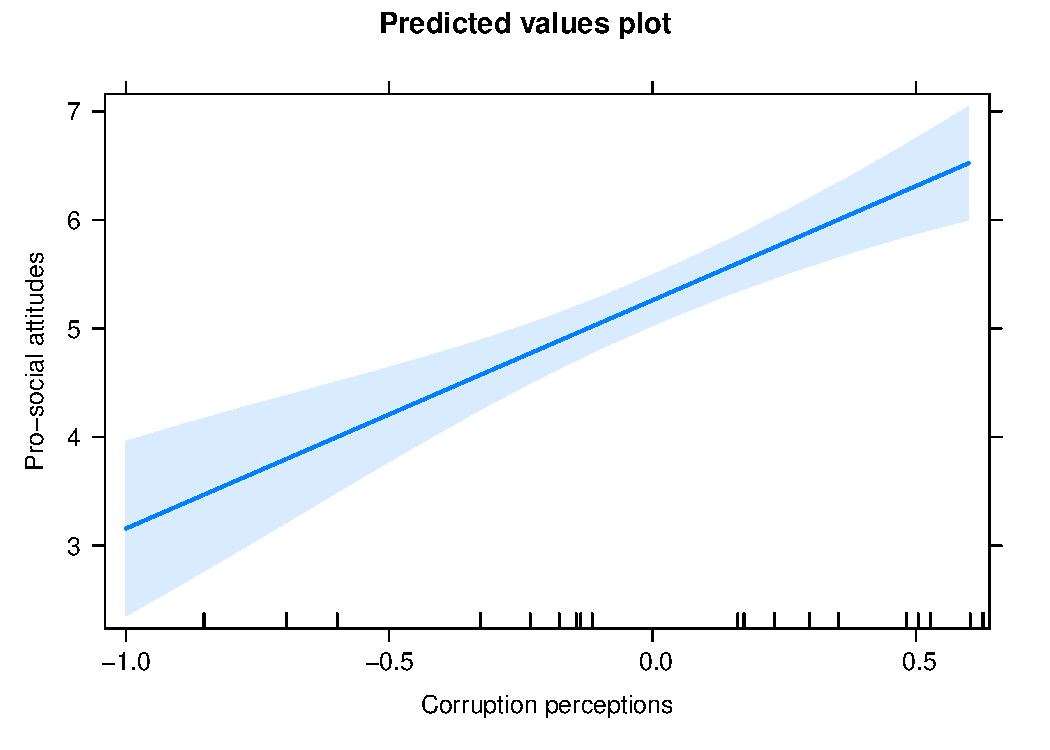
\includegraphics[width=0.95\textwidth]{../../05-graphs/Supplem-05.pdf}
  \caption{Predicted values with \texttt{effects} package}
  \label{fig:fig-03}
\end{figure}

Had we obtained any significant results from the interaction model (in Model 4), we would probably have produced a marginal effects plot as well, to show how the effect of education varies depending on CPI.\footnote{Remember that an interaction is symmetric, so the coefficient can be interpreted as how the effect of education varies across contexts with different CPIs, or how the effect of CPI is different for individuals with different levels of education. The interpretation depends mostly on how you have framed your theoretical questions.} Since we did not get a significant coefficient there is little to interpret, although for the sake of practice we can also produce this plot as well.

\begin{knitrout}
\definecolor{shadecolor}{rgb}{0.969, 0.969, 0.969}\color{fgcolor}\begin{kframe}
\begin{alltt}
\hlkwd{quantile}\hlstd{(df_sub}\hlopt{$}\hlstd{cpi.cgm,} \hlkwd{c}\hlstd{(}\hlnum{0.1}\hlstd{,} \hlnum{0.5}\hlstd{,} \hlnum{0.9}\hlstd{))}
\hlkwd{plot}\hlstd{(}\hlkwd{effect}\hlstd{(}\hlstr{"edu.cwc:cpi.cgm"}\hlstd{, model4,}
     \hlkwc{xlevels} \hlstd{=} \hlkwd{list}\hlstd{(}\hlkwc{cpi.cgm} \hlstd{=} \hlkwd{c}\hlstd{(}\hlopt{-}\hlnum{0.85}\hlstd{,} \hlnum{0.15}\hlstd{,} \hlnum{0.65}\hlstd{))),}
     \hlkwc{main} \hlstd{=} \hlstr{"Marginal effects plot"}\hlstd{,}
     \hlkwc{xlab} \hlstd{=} \hlstr{"Corruption perceptions"}\hlstd{,}
     \hlkwc{ylab} \hlstd{=} \hlstr{"Effect of education on pro-social behavior"}\hlstd{)}
\end{alltt}
\end{kframe}
\end{knitrout}



\begin{figure}[!ht]
  \centering
  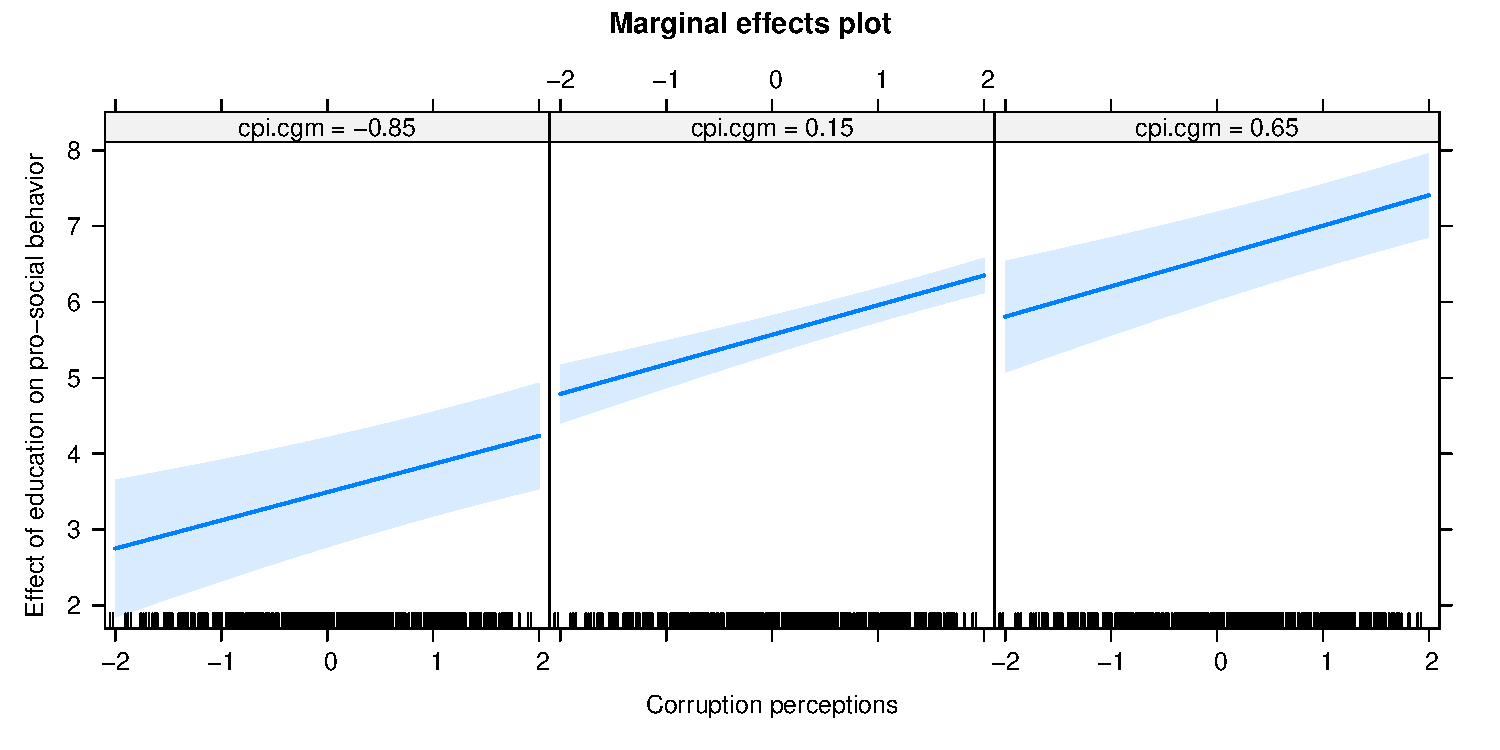
\includegraphics[width=0.95\textwidth]{../../05-graphs/Supplem-06.pdf}
  \caption{Marginal effects plot with \texttt{effects} package}
  \label{fig:fig-04}
\end{figure}

As can be seen from Figure~\ref{fig:fig-04}, there is no real distinction between the effect of education at different levels of CPI. In a sense this is what the non-significant coefficient of the interaction term told us as well.

\end{document}
